\documentclass[final,table,14pt,svgnames]{beamer}
\usepackage[orientation=lanscape,size=a4,scale=4]{beamerposter}
\setbeamertemplate{navigation symbols}{}
\usepackage{graphicx}
\usepackage{tikz}
\usepackage{marvosym}
\usepackage{pgfpages}
\usepackage{hyperref}
\usepackage{fontawesome}
\usepackage{xcolor}
\usepackage{stackengine}
\usepackage{shadowtext}
\usepackage[export]{adjustbox}
%\usefonttheme{serif}
\urlstyle{sf}


\tikzstyle{na} = [baseline=-.5ex]
\usetikzlibrary{arrows,shapes,backgrounds}
\tikzstyle{every picture}+=[remember picture]
\usetikzlibrary{spy}

\newfontfamily\oldschool[Path = /home/ctroupin/.fonts/]{ScorchedEarthDEMO-KCFonts.otf}
\newfontfamily\titlet[Path = /home/ctroupin/.fonts/]{aliens and cows_trial.ttf}

\usepackage{fontspec}
\defaultfontfeatures{Ligatures=TeX}

\definecolor{bluegher}{RGB}{4,99,128}  		% blue 
\definecolor{greygher}{RGB}{50, 50, 50}  	% grey 
\definecolor{greytext}{RGB}{100, 100, 100}  	% grey 
\definecolor{redgher}{RGB}{189, 33, 5}  	% red 
\definecolor{greybackground}{RGB}{235, 235, 235}

\hypersetup{colorlinks,linkcolor=,urlcolor=bluegher}

\setbeamerfont{title}{size=\huge,family=\titlet}
\setbeamerfont{subtitle}{size=\LARGE,series=\oldschool}
\setbeamerfont{date}{size=\scriptsize}
\setbeamerfont{projected text}{size=\normalsize,series=\oldschool}

\setbeamercolor{title}{fg=bluegher}
\setbeamercolor{projected text}{fg=bluegher}
\setbeamercolor{subtitle}{bg=bluegher,fg=white}
\setbeamercolor{projected text}{fg=bluegher,bg=white}

\setbeamersize{text margin left=.1cm, text margin right=1cm} %new code


   
% ------------------------------------------------
% LENGTH DEFINITIONS
%-------------------------------------------------
%\setlength{\textwidth}{24cm}
%\setlength{\textheight}{28cm}
\setbeamersize{text margin left=10pt,text margin right=10pt}

\newsavebox{\ximagebox}
\newlength{\ximageheight}
\newsavebox{\xglyphbox}
\newlength{\xglyphheight}
\newcommand{\xbox}[1]%
   {\savebox{\ximagebox}{#1}%
    \settoheight{\ximageheight}{\usebox{\ximagebox}}%
    \savebox{\xglyphbox}{\char32}%
    \settoheight{\xglyphheight}{\usebox{\xglyphbox}}%
    \raisebox{\ximageheight}[0pt][0pt]{\raisebox{-\xglyphheight}[0pt][0pt]{%
      \makebox[0pt][l]{\usebox{\xglyphbox}}}}%
    \usebox{\ximagebox}%
    \raisebox{0pt}[0pt][0pt]{\makebox[0pt][r]{\usebox{\xglyphbox}}}}
    

\newcommand{\seplogo}{\hspace{.45cm}}
\newcommand{\figheight}{.0625\textheight}
\newcommand{\figheightB}{.07\textheight}
\newcommand{\putlogo}[1]{\includegraphics[height=\figheight]{#1}}
\newcommand{\putlogolink}[2]{\href{#1}{\xbox{\includegraphics[height=\figheight]{#2}}}}
\newcommand{\putlogoB}[1]{\includegraphics[height=\figheightB]{#1}}
\newcommand{\sepauthor}{$\bullet$~}

\DeclareGraphicsExtensions{.eps,.JPG,.jpg,.pdf,.png,.PNG,.jpeg}
\graphicspath{
{./logos/},
}

\parindent 0cm

\usebackgroundtemplate{\tikz\node[opacity=0.33]{\parbox[c][.3\paperheight][c]{\paperwidth}{\hspace{-.25cm}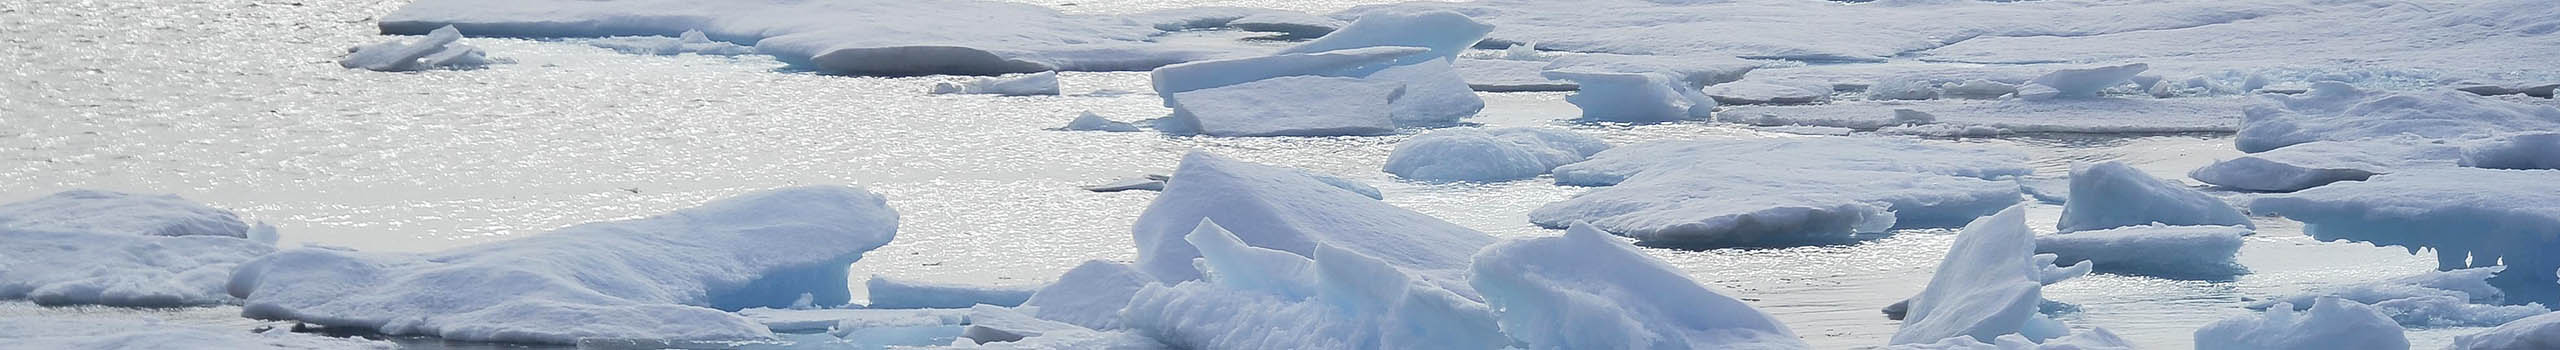
\includegraphics[width=1.05\paperwidth]{images/banner_oceano_chimique.jpg}}};}

% These lines to keep good colors when viewed with Acrobat Reader
\makeatletter%
\special{pdf: put @thispage <</Group << /S /Transparency /I true /CS /DeviceRGB>> >>}%
\makeatother%

\author{}
%\url{www.socib.es}}
\subtitle{facing changes}
\title{Polar Ocean}
\date{6--10~May, 2019}

\begin{document}
\def\stackalignment{l}

\begin{frame}[fragile, t]
\centering

% Background rectangles
\begin{tikzpicture}[remember picture,overlay]%

%\draw[step=1cm,lightgray,very thin] (-11,-24) grid (20, 20);
 
\coordinate (tp1) at ([yshift=-.5cm, xshift=.5cm]current page.north west);
\coordinate (tp2) at ([yshift=-6cm, xshift=.5cm]current page.north west);
\coordinate (tp3) at ([yshift=-6cm, xshift=-.5cm]current page.north east);
\coordinate (tp4) at ([yshift=-.5cm, xshift=-.5cm]current page.north east);

\coordinate (tp5) at (current page.south west);
\coordinate (tp6) at ([yshift=\figheight+1.2cm	]current page.south west);
\coordinate (tp7) at ([yshift=\figheight+1.2cm]current page.south east);
\coordinate (tp8) at (current page.south east);

%\filldraw[draw=none,fill=DarkTurquoise,opacity=0.35] (tp1)--(tp2)--(tp3)--(tp4)--cycle;

\filldraw[draw=greybackground,fill=greybackground,opacity=0.7] (tp5)--(tp6)--(tp7)--(tp8)--cycle;

%\shade[top color=bluegher,bottom color=white,opacity=0.7] (tp1)--(tp2)--(tp3)--(tp4)--cycle;

\node[anchor=north east,yshift=-35pt,xshift=-.5cm] at (current page.north east) {
\includegraphics[height=.05\textheight]{logo_colloquium}};

\end{tikzpicture}

\begin{center}


{\usebeamerfont{title}\inserttitle}

\vspace{.05cm}

\shadowoffsetx{3pt}\shadowoffsety{3pt}
\usebeamerfont{subtitle}\usebeamercolor[fg]{subtitle}\usebeamercolor[bg]{subtitle}\shadowtext{\insertsubtitle}

\end{center}


\vspace*{1cm}
\footnotesize 51st International Liege Colloquium on Ocean Dynamics
\vspace*{.5cm}


\begin{figure}
\centering
\includegraphics[width=.5\textwidth,cfbox=bluegher 2pt 2pt]{../figures/background2019.jpg}%\includegraphics[width=.5\textwidth]{clq_background2}
%\includegraphics[width=\textwidth]{timeseries}
\end{figure}

{\scriptsize
\textcolor{greygher}{\faCalendarCheckO~~\insertdate}\\
\textcolor{bluegher}{{\faHome}~~\url{http://labos.ulg.ac.be/gher/home/colloquium/}}\\
\textcolor{greygher}{\faMapPin~~University of Liège - Place du 20-Août, 7 - 4000 Liège - Belgium}\\
\fcolorbox{black}{bluegher}{\textcolor{white}{\faWarning~~Deadline for abstracts: 15th March 2019}}
}

\vspace{2cm}


%{\scriptsize 
%\href{http://modb.oce.ulg.ac.be/colloquium/2016/#col_travel_grants}{Travel support}: please visit the colloquium web page
%}
\vfill


%-------------------------------------
% Place the logo for the sponsors here
%-------------------------------------

\vfill

\begin{tikzpicture}[remember picture,overlay]
  \node[anchor=south] at (current page.south) {
  \begin{columns}[totalwidth=1.\textwidth,c]
\column{.265\textwidth}
\scriptsize
\putlogolink{http://www.ulg.ac.be}{logo_uliege} \putlogolink{http://labos.ulg.ac.be/oceanologie/}{images/logo_oceano_short} 
\seplogo \putlogolink{http://modb.oce.ulg.ac.be/}{logo_gher}
\column{.02\textwidth}
~
\column{.7\textwidth}
\scriptsize
\putlogolink{http://www.wallonie.be/}{coq_wallon} \seplogo \putlogolink{http://www.fnrs.be/}{logo_fnrs}\seplogo \putlogolink{https://www.belspo.be/}{logo_belspo} \hfill \stackanchor{\textcolor{greygher}{\faTwitter~~~@GHER\_ULg}}{\textcolor{bluegher}{\faHashtag~~~LiegeOcean2019}} \hspace*{1cm}
\end{columns}
};
\end{tikzpicture}



\end{frame}



\end{document}
